%!TEX TS-program = xelatex
%!TEX options = -aux-directory=Debug -shell-escape -file-line-error -interaction=nonstopmode -halt-on-error -synctex=1 "%DOC%"
\documentclass{article}
\input{LaTeX-Submodule/template.tex}

% Additional packages & macros
\DeclareMathOperator{\sgn}{sgn}
\DeclareMathOperator{\sinc}{sinc}

% Header and footer
\newcommand{\unitName}{Signal Analysis}
\newcommand{\unitTime}{Semester 2, 2022}
\newcommand{\unitCoordinator}{Prof Wageeh Boles}
\newcommand{\documentAuthors}{Tarang Janawalkar}

\fancyhead[L]{\unitName}
\fancyhead[R]{\leftmark}
\fancyfoot[C]{\thepage}

% Copyright
\usepackage[
    type={CC},
    modifier={by-nc-sa},
    version={4.0},
    imagewidth={5em},
    hyphenation={raggedright}
]{doclicense}

\date{}

\begin{document}
%
\begin{titlepage}
    \vspace*{\fill}
    \begin{center}
        \LARGE{\textbf{\unitName}} \\[0.1in]
        \normalsize{\unitTime} \\[0.2in]
        \normalsize\textit{\unitCoordinator} \\[0.2in]
        \documentAuthors
    \end{center}
    \vspace*{\fill}
    \doclicenseThis
    \thispagestyle{empty}
\end{titlepage}
\newpage
%
\tableofcontents
\newpage
%
\section{Properties of Mathematical Functions}
\subsection{Even and Odd Functions}
\begin{definition}[Even function]
    A function \(x\left( t \right)\) is even if
    \begin{equation*}
        x\left( -t \right) = x\left( t \right)
    \end{equation*}
    for all \(t\) in the functions domain. Even functions are symmetric about the vertical axis.
\end{definition}
\begin{definition}[Odd function]
    A function \(x\left( t \right)\) is odd if
    \begin{equation*}
        x\left( -t \right) = -x\left( t \right)
    \end{equation*}
    for all \(t\) in the functions domain. Odd functions are symmetric about the origin.
\end{definition}
\subsubsection{Integrating Even and Odd Functions}
When integrating an \textbf{even} function \(x\left( t \right)\) over the domain \(\interval{-T}{T}\):
\begin{equation*}
    \int_{-T}^T x\left( t \right) \odif{t} = 2 \int_0^T x\left( t \right) \odif{t}.
\end{equation*}
Similarly, when integrating an \textbf{odd} function \(x\left( t \right)\) over the domain \(\interval{-T}{T}\):
\begin{equation*}
    \int_{-T}^T x\left( t \right) \odif{t} = 0.
\end{equation*}
\subsubsection{Product of Even and Odd Functions}
\begin{enumerate}
    \item The product of an \textbf{even} function with an \textbf{even} function, is an \textbf{even} function.

          Let \(f\left( t \right)\) and \(g\left( t \right)\) be even functions, and let \(h\left( t \right) = f\left( t \right) g\left( t \right)\),
          \begin{equation*}
              h\left( -t \right) = f\left( -t \right) g\left( -t \right) = f\left( t \right) g\left( t \right) = h\left( t \right).
          \end{equation*}
    \item The product of an \textbf{even} function with an \textbf{odd} function, is an \textbf{odd} function.

          Let \(f\left( t \right)\) be an even function and \(g\left( t \right)\) be an odd function, and let \(h\left( t \right) = f\left( t \right) g\left( t \right)\),
          \begin{equation*}
              h\left( -t \right) = f\left( -t \right) g\left( -t \right) = \left( -f\left( t \right) \right) g\left( t \right) = -h\left( t \right).
          \end{equation*}
    \item The product of an \textbf{odd} function with an \textbf{odd} function, is an \textbf{even} function.

          Let \(f\left( t \right)\) and \(g\left( t \right)\) be odd functions, and let \(h\left( t \right) = f\left( t \right) g\left( t \right)\),
          \begin{equation*}
              h\left( -t \right) = f\left( -t \right) g\left( -t \right) = \left( -f\left( t \right) \right) \left( -g\left( t \right) \right) = f\left( t \right) g\left( t \right) = h\left( t \right).
          \end{equation*}
\end{enumerate}
\subsection{Orthogonality}
\begin{definition}[Inner product]
    An inner product generalises the dot product in general vector spaces.

    In particular, for the function space \(\mathscr{F}\left( \interval{a}{b} \right)\), where \(t \in \interval{a}{b}\),
    the inner product is defined as the following:
    \begin{equation*}
        \abracket*{f,\: g} = \int_a^b f\left( t \right) g\left( t \right) \odif{t}
    \end{equation*}
    for \(f,\: g \in \mathscr{F}\left( \interval{a}{b} \right)\).
\end{definition}
\begin{definition}[Orthogonality]
    Given an inner product space, two vectors are orthogonal iff
    \begin{equation*}
        \abracket*{f,\: g} = 0.
    \end{equation*}
\end{definition}
\subsection{Orthogonality of Trigonometric Functions}
Consider the inner product between the sine and cosine functions on the interval \(\interval{-T}{T}\).
\begin{equation*}
    \abracket*{\sin{\left( t \right)},\: \cos{\left( t \right)}} = \int_{-T}^T \sin{\left( t \right)} \cos{\left( t \right)} \odif{t} = 0
\end{equation*}
as the integrand is an odd function.
\subsection{Integrals of Trigonometric Functions}
For \(n \in \Z\):
\begin{align*}
    \int_{t_0}^{t_0 + T} \sin{\left( 2\pi n f_0 t \right)} \odif{t} & = - \frac{1}{2\pi n f_0} \left[ \cos{\left( 2\pi n f_0 t \right)} \right]_{t_0}^{t_0 + T}                                                        \\
                                                                    & = - \frac{1}{2\pi n f_0} \left[ \cos{\left( \frac{2\pi n}{T} \left( t_0 + T \right) \right)} - \cos{\left( \frac{2\pi n}{T} t_0 \right)} \right] \\
                                                                    & = - \frac{1}{2\pi n f_0} \left[ \cos{\left( \frac{2\pi n}{T} t_0 + 2\pi n \right)} - \cos{\left( \frac{2\pi n}{T} t_0 \right)} \right]           \\
                                                                    & = - \frac{1}{2\pi n f_0} \left[ \cos{\left( \frac{2\pi n}{T} t_0 \right)} - \cos{\left( \frac{2\pi n}{T} t_0 \right)} \right]                    \\
                                                                    & = - \frac{1}{2\pi n f_0} \left[ 0 \right]                                                                                                        \\
                                                                    & = 0.
\end{align*}
\begin{align*}
    \int_{t_0}^{t_0 + T} \cos{\left( 2\pi n f_0 t \right)} \odif{t} & = \frac{1}{2\pi n f_0} \left[ \sin{\left( 2\pi n f_0 t \right)} \right]_{t_0}^{t_0 + T}                                                        \\
                                                                    & = \frac{1}{2\pi n f_0} \left[ \sin{\left( \frac{2\pi n}{T} \left( t_0 + T \right) \right)} - \sin{\left( \frac{2\pi n}{T} t_0 \right)} \right] \\
                                                                    & = \frac{1}{2\pi n f_0} \left[ \sin{\left( \frac{2\pi n}{T} t_0 + 2\pi n \right)} - \sin{\left( \frac{2\pi n}{T} t_0 \right)} \right]           \\
                                                                    & = \frac{1}{2\pi n f_0} \left[ \sin{\left( \frac{2\pi n}{T} t_0 \right)} - \sin{\left( \frac{2\pi n}{T} t_0 \right)} \right]                    \\
                                                                    & = \frac{1}{2\pi n f_0} \left[ 0 \right]                                                                                                        \\
                                                                    & = 0.
\end{align*}
\subsubsection{Product of Trigonometric Functions}
Recall the Werner formulas:
\begin{gather*}
    2 \cos{\left( \alpha \right)} \cos{\left( \beta \right)} = \cos{\left( \alpha - \beta \right)} + \cos{\left( \alpha + \beta \right)} \\
    2 \sin{\left( \alpha \right)} \sin{\left( \beta \right)} = \cos{\left( \alpha - \beta \right)} - \cos{\left( \alpha + \beta \right)} \\
    2 \sin{\left( \alpha \right)} \cos{\left( \beta \right)} = \sin{\left( \alpha - \beta \right)} + \sin{\left( \alpha + \beta \right)}
\end{gather*}
For \(n,\: m \in \N\),

\underline{Product of two cosine functions:}
\begin{equation*}
    \int_{t_0}^{t_0 + T} \cos{\left( 2\pi n f_0 t \right)} \cos{\left( 2\pi m f_0 t \right)} \odif{t} = \frac{1}{2} \int_{t_0}^{t_0 + T} \cos{\left( 2 \pi \left( n - m \right) f_0 t \right)} + \cos{\left( 2 \pi \left( n + m \right) f_0 t \right)} \odif{t}
\end{equation*}
\(n = m \implies n - m = 0\) and \(\left( n + m \right) \in \Z\), so that the integral of the second
term is \(0\), and the integral of the first term results in \(\frac{T}{2}\).

\(n \neq m \implies \left( n - m \right),\: \left( n + m \right) \in \Z\) so that both terms evaluate to \(0\) when integrated separately.
\begin{equation*}
    \int_{t_0}^{t_0 + T} \cos{\left( 2\pi n f_0 t \right)} \cos{\left( 2\pi m f_0 t \right)} \odif{t} = \begin{cases}
        \frac{T}{2}, & n = m     \\
        0,           & n \neq m.
    \end{cases}
\end{equation*}
\underline{Product of two sine functions:}
\begin{equation*}
    \int_{t_0}^{t_0 + T} \sin{\left( 2\pi n f_0 t \right)} \sin{\left( 2\pi m f_0 t \right)} \odif{t} = \frac{1}{2} \int_{t_0}^{t_0 + T} \cos{\left( 2 \pi \left( n - m \right) f_0 t \right)} - \cos{\left( 2 \pi \left( n + m \right) f_0 t \right)} \odif{t}
\end{equation*}
By the same argument as before,
\begin{equation*}
    \int_{t_0}^{t_0 + T} \sin{\left( 2\pi n f_0 t \right)} \sin{\left( 2\pi m f_0 t \right)} \odif{t} = \begin{cases}
        \frac{T}{2}, & n = m     \\
        0,           & n \neq m.
    \end{cases}
\end{equation*}
\underline{Product of sine and cosine functions:}
\begin{equation*}
    \int_{t_0}^{t_0 + T} \sin{\left( 2\pi n f_0 t \right)} \cos{\left( 2\pi m f_0 t \right)} \odif{t} = \frac{1}{2} \int_{t_0}^{t_0 + T} \sin{\left( 2 \pi \left( n - m \right) f_0 t \right)} + \sin{\left( 2 \pi \left( n + m \right) f_0 t \right)} \odif{t}
\end{equation*}
\(n = m \implies n - m = 0\) and \(\left( n + m \right) \in \Z\), so that the integral reduces to \(0\).

\(n \neq m \implies \left( n - m \right),\: \left( n + m \right) \in \Z\) so that both terms evaluate to \(0\) when integrated separately.
\begin{equation*}
    \int_{t_0}^{t_0 + T} \sin{\left( 2\pi n f_0 t \right)} \cos{\left( 2\pi m f_0 t \right)} \odif{t} = 0.
\end{equation*}
\section{Fourier Series}
\subsection{Fourier Series Expansion}
The \textbf{Fourier Series Expansion} of a function \(x\left( t \right)\) on the interval \(\interval{t_0}{t_0 + T}\)
is given by
\begin{equation*}
    x_F\left( t \right) = a_0 + \sum_{n = 1}^\infty \left( a_n \cos{\left( 2\pi n f_0 t \right)} + b_n \sin{\left( 2\pi n f_0 t \right)} \right)
\end{equation*}
where \(n \in \Z^{+}\) and \(f_0 = \frac{1}{T}\). The coefficients are given by
\begin{align*}
    a_0 & = \frac{1}{T} \int_{t_0}^{t_0 + T} x\left( t \right) \odif{t}                                   \\
    a_n & = \frac{2}{T} \int_{t_0}^{t_0 + T} x\left( t \right) \cos{\left( 2\pi n f_0 t \right)} \odif{t} \\
    b_n & = \frac{2}{T} \int_{t_0}^{t_0 + T} x\left( t \right) \sin{\left( 2\pi n f_0 t \right)} \odif{t}
\end{align*}
\begin{proof}
    Let \(m \in \N\).

    For the coefficient \(a_0\), integrate the function \(x\left( t \right)\) over the interval \(\interval{t_0}{t_0 + T}\).
    \begin{align*}
        \int_{t_0}^{t_0 + T} x\left( t \right) \odif{t} & = \int_{t_0}^{t_0 + T} a_0 \odif{t} + \sum_{n = 1}^\infty a_n \cancelto{0}{\int_{t_0}^{t_0 + T} \cos{\left( 2 \pi n f_0 t \right)} \odif{t}} + \sum_{n = 1}^\infty b_n \cancelto{0}{\int_{t_0}^{t_0 + T} \sin{\left( 2 \pi n f_0 t \right)} \odif{t}} \\
        \int_{t_0}^{t_0 + T} x\left( t \right) \odif{t} & = a_0 T                                                                                                                                                                                                                                               \\
        a_0                                             & = \frac{1}{T} \int_{t_0}^{t_0 + T} x\left( t \right) \odif{t}
    \end{align*}
    so that \(a_0\) represents the average value of \(x\) on \(\interval{t_0}{t_0 + T}\). This coefficient also
    represents the DC component of a signal.

    For coefficients \(a_m\), multiply the equation by \(\cos{\left( 2 \pi m f_0 t \right)}\) before integrating.
    \begin{align*}
        x\left( t \right) \cos{\left( 2 \pi m f_0 t \right)}                               & = \begin{aligned}[t]
                                                                                                    & a_0 \cos{\left( 2 \pi m f_0 t \right)}                                                          \\
                                                                                                    & + \sum_{n = 1}^\infty a_n \cos{\left( 2 \pi n f_0 t \right)} \cos{\left( 2 \pi m f_0 t \right)} \\
                                                                                                    & + \sum_{n = 1}^\infty b_n \sin{\left( 2 \pi n f_0 t \right)} \cos{\left( 2 \pi m f_0 t \right)}
                                                                                               \end{aligned}                                                    \\
        \int_{t_0}^{t_0 + T} x\left( t \right) \cos{\left( 2 \pi m f_0 t \right)} \odif{t} & = \begin{aligned}[t]
                                                                                                    & a_0 \cancelto{0}{\int_{t_0}^{t_0 + T} \cos{\left( 2 \pi m f_0 t \right)} \odif{t}}                                                          \\
                                                                                                    & + \sum_{n = 1}^\infty a_n \int_{t_0}^{t_0 + T} \cos{\left( 2 \pi n f_0 t \right)} \cos{\left( 2 \pi m f_0 t \right)} \odif{t}               \\
                                                                                                    & + \sum_{n = 1}^\infty b_n \cancelto{0}{\int_{t_0}^{t_0 + T} \sin{\left( 2 \pi n f_0 t \right)} \cos{\left( 2 \pi m f_0 t \right)} \odif{t}}
                                                                                               \end{aligned} \\
        \int_{t_0}^{t_0 + T} x\left( t \right) \cos{\left( 2 \pi m f_0 t \right)} \odif{t} & = a_m \frac{T}{2}                                                                                                                                       \\
        a_m                                                                                & = \frac{2}{T} \int_{t_0}^{t_0 + T} x\left( t \right) \cos{\left( 2 \pi m f_0 t \right)} \odif{t}
    \end{align*}

    For coefficients \(b_m\), multiply the equation by \(\sin{\left( 2 \pi m f_0 t \right)}\) before integrating.
    \begin{align*}
        x\left( t \right) \sin{\left( 2 \pi m f_0 t \right)}                               & = \begin{aligned}[t]
                                                                                                    & a_0 \sin{\left( 2 \pi m f_0 t \right)}                                                          \\
                                                                                                    & + \sum_{n = 1}^\infty a_n \cos{\left( 2 \pi n f_0 t \right)} \sin{\left( 2 \pi m f_0 t \right)} \\
                                                                                                    & + \sum_{n = 1}^\infty b_n \sin{\left( 2 \pi n f_0 t \right)} \sin{\left( 2 \pi m f_0 t \right)}
                                                                                               \end{aligned}                                                    \\
        \int_{t_0}^{t_0 + T} x\left( t \right) \sin{\left( 2 \pi m f_0 t \right)} \odif{t} & = \begin{aligned}[t]
                                                                                                    & a_0 \cancelto{0}{\int_{t_0}^{t_0 + T} \sin{\left( 2 \pi m f_0 t \right)} \odif{t}}                                                          \\
                                                                                                    & + \sum_{n = 1}^\infty a_n \cancelto{0}{\int_{t_0}^{t_0 + T} \cos{\left( 2 \pi n f_0 t \right)} \sin{\left( 2 \pi m f_0 t \right)} \odif{t}} \\
                                                                                                    & + \sum_{n = 1}^\infty b_n \int_{t_0}^{t_0 + T} \sin{\left( 2 \pi n f_0 t \right)} \sin{\left( 2 \pi m f_0 t \right)} \odif{t}
                                                                                               \end{aligned} \\
        \int_{t_0}^{t_0 + T} x\left( t \right) \sin{\left( 2 \pi m f_0 t \right)} \odif{t} & = b_m \frac{T}{2}                                                                                                                                       \\
        b_m                                                                                & = \frac{2}{T} \int_{t_0}^{t_0 + T} x\left( t \right) \sin{\left( 2 \pi m f_0 t \right)} \odif{t}
    \end{align*}
\end{proof}
\subsubsection{Convergence of a Fourier Series}
If \(x\left( t \right)\) is piecewise smooth on \(\interval{t_0}{t_0 + L}\), \(x_F\left( t \right)\)
converges to
\begin{equation*}
    x_F\left( t \right) = \lim_{\epsilon \to 0^{+}} \frac{x\left( t + \epsilon \right) + x\left( t - \epsilon \right)}{2}
\end{equation*}
that is, \(x = x_F\), except at discontinuities, where \(f_F\) is equal to the point halfway between the left- and right-handed limits.
\subsubsection{Periodicity of a Fourier Series}
If \(x\) is non-periodic, \(x_F\) converges to the periodic extension of \(x\). The endpoints may converge non-uniformly,
corresponding to jump discontinuities in the periodic extension of \(x\).
\subsection{Fourier Cosine Series}
Consider the Fourier series expansion of an even function \(x\) on the interval \(\interval{-\frac{T}{2}}{\frac{T}{2}}\), i.e., \(t_0 = -\frac{T}{2}\).
In this case,
\begin{equation*}
    b_n = \frac{2}{T} \int_{-\frac{T}{2}}^{\frac{T}{2}} x\left( t \right) \sin{\left( 2\pi n f_0 t \right)} \odif{t} = 0
\end{equation*}
and the Fourier series is a ``Fourier cosine series'', given by:
\begin{equation*}
    x_c\left( t \right) = a_0 + \sum_{n = 1}^\infty a_n \cos{\left( 2\pi n f_0 t \right)}
\end{equation*}
with coefficients
\begin{align*}
    a_0 & = \frac{1}{T} \int_{-\frac{T}{2}}^{\frac{T}{2}} x\left( t \right) \odif{t}                                    = \frac{2}{T} \int_0^{\frac{T}{2}} x\left( t \right) \odif{t}                                    \\
    a_n & = \frac{2}{T} \int_{-\frac{T}{2}}^{\frac{T}{2}} x\left( t \right) \cos{\left( 2 \pi n f_0 t \right)} \odif{t} = \frac{4}{T} \int_0^{\frac{T}{2}} x\left( t \right) \cos{\left( 2\pi n f_0 t \right)} \odif{t}.
\end{align*}
\subsection{Fourier Sine Series}
Consider the Fourier series expansion of an odd function \(x\) on the interval \(\interval{-\frac{T}{2}}{\frac{T}{2}}\).
In this case
\begin{equation*}
    b_n = \frac{2}{T} \int_{-\frac{T}{2}}^{\frac{T}{2}} x\left( t \right) \sin{\left( 2\pi n f_0 t \right)} \odif{t} = 0
\end{equation*}
and the Fourier series is a ``Fourier sine series'', given by:
\begin{equation*}
    x_s\left( t \right) = \sum_{n = 1}^\infty b_n \sin{\left( 2\pi n f_0 t \right)}
\end{equation*}
with coefficients
\begin{equation*}
    b_n = \frac{2}{T} \int_{-\frac{T}{2}}^{\frac{T}{2}} x\left( t \right) \sin{\left( 2 \pi n f_0 t \right)} \odif{t} = \frac{4}{T} \int_0^{\frac{T}{2}} x\left( t \right) \sin{\left( 2\pi n f_0 t \right)} \odif{t}.
\end{equation*}
\section{Complex Fourier Series}
\begin{definition}
    The \textbf{Complex Fourier Series Expansion} is a concise form of the Fourier series expansion that uses complex exponentials with a single unknown coefficient.
    \begin{equation*}
        x_C\left( t \right) = \sum_{n = -\infty}^\infty c_n e^{j 2\pi n f_0 t}
    \end{equation*}
    where
    \begin{equation*}
        c_n = \frac{1}{T} \int_{t_0}^{t_0 + T} x\left( t \right) e^{-j 2\pi n f_0 t} \odif{t}.
    \end{equation*}
    for \(n \in \Z\) and \(f_0 = \frac{1}{T}\).
\end{definition}
To determine the complex Fourier series expansion consider the following identities:
\begin{align*}
    \cos{\left( \theta \right)} & = \frac{e^{j \theta} + e^{-j \theta}}{2}     \\
    \sin{\left( \theta \right)} & = -j \frac{e^{j \theta} - e^{-j \theta}}{2}.
\end{align*}
By substituting these identities into the Fourier series expansion summand, we obtain:
\begin{align*}
    a_n \cos{\left( 2\pi n f_0 t \right)} + b_n \sin{\left( 2\pi n f_0 t \right)} & = a_n \frac{e^{j 2\pi n f_0 t} + e^{-j 2\pi n f_0 t}}{2} -j b_n \frac{e^{j 2\pi n f_0 t} - e^{-j 2\pi n f_0 t}}{2} \\
                                                                                  & = \frac{a_n - j b_n}{2} e^{j 2\pi n f_0 t} + \frac{a_n + j b_n}{2} e^{-j 2\pi n f_0 t}
\end{align*}
Let \(c_n = \frac{a_n - j b_n}{2}\) and \(c_n^\ast = \frac{a_n + j b_n}{2}\) (we will see how this simplifies later).
Using the definitions for \(a_n\) and \(b_n\):
\begin{align*}
    c_n & = \frac{1}{2} \left( a_n - j b_n \right)                                                                                                            \\
        & = \frac{1}{T} \int_{t_0}^{t_0 + T} x\left( t \right) \left( \cos{\left( 2\pi n f_0 t \right)} -j \sin{\left( 2\pi n f_0 t \right)} \right) \odif{t} \\
        & = \frac{1}{T} \int_{t_0}^{t_0 + T} x\left( t \right) e^{-j 2\pi n f_0 t} \odif{t}
\end{align*}
\begin{align*}
    c_n^\ast & = \frac{1}{2} \left( a_n + j b_n \right)                                                                                                             \\
             & = \frac{1}{T} \int_{t_0}^{t_0 + T} x\left( t \right) \left( \cos{\left( 2\pi n f_0 t \right)} + j \sin{\left( 2\pi n f_0 t \right)} \right) \odif{t} \\
             & = \frac{1}{T} \int_{t_0}^{t_0 + T} x\left( t \right) e^{j 2\pi n f_0 t} \odif{t}                                                                     \\
             & = c_{-n}
\end{align*}
Let \(c_0 = a_0\), so that
\begin{align*}
    x_C\left( t \right) & = a_0 + \sum_{n = 1}^\infty \left( a_n \cos{\left( 2\pi n f_0 t \right)} + b_n \sin{\left( 2\pi n f_0 t \right)} \right) \\
                        & = c_0 + \sum_{n = 1}^\infty \left( c_n e^{j 2\pi n f_0 t} + c_{-n} e^{-j 2\pi n f_0 t} \right)                           \\
                        & = c_0 + \sum_{n = 1}^\infty c_n e^{j 2\pi n f_0 t} + \sum_{n = 1}^\infty c_{-n} e^{-j 2\pi n f_0 t}                      \\
                        & = c_0 + \sum_{n = 1}^\infty c_n e^{j 2\pi n f_0 t} + \sum_{n = -\infty}^{-1} c_{n} e^{j 2\pi n f_0 t}                    \\
                        & = \sum_{n = -\infty}^\infty c_n e^{j 2\pi n f_0 t}.
\end{align*}
\subsection{Converting between Fourier Series Representations}
Given the Trigonometric and Exponential (Complex) Fourier Series Representations (FSR),
we can develop a relationship between the coefficients \(a_n\), \(b_n\), and \(c_n\) by:
\begin{align*}
    a_0 & = c_0                           \\
    a_n & = c_n + c_{-n}                  \\
    b_n & = j \left( c_n - c_{-n} \right)
\end{align*}
and in the reverse direction:
\begin{align*}
    c_{-n} & = \frac{a_n + j b_n}{2}  \\
    c_0    & = a_0                    \\
    c_n    & = \frac{a_n - j b_n}{2}.
\end{align*}
\subsection{Magnitude and Phase Spectra}
As \(c_n\) is a complex number, consider the polar representation of \(c_n\):
\begin{equation*}
    c_n = \abs*{c_n} e^{j \theta_n}
\end{equation*}
so that the \textbf{magnitude spectra} is given by \(\abs*{c_n}\) and the \textbf{phase spectra} is given by \(\theta_n\).

The plot of \(\abs*{c_n}\) against \(n\) is called the ``magnitude spectrum'' of \(x\left( t \right)\) and
the plot of \(\theta_n\) against \(n\) is called the ``phase spectrum'' of \(x\left( t \right)\).
\begin{theorem}[Spectra of a real signal]
    Given any real function \(x\left( t \right)\), the magnitude spectrum is always an even function,
    and the phase spectrum is always an odd function.
\end{theorem}
\begin{proof}
    Given a real function \(x\left( t \right)\), the exponential Fourier series is given by,
    \begin{equation*}
        x_C\left( t \right) = \sum_{n = -\infty}^\infty c_n e^{j 2\pi n f_0 t}
    \end{equation*}
    this is equivalent to
    \begin{equation*}
        x_C\left( t \right) = \sum_{n = -\infty}^\infty c_{-n} e^{-j 2\pi n f_0 t}.
    \end{equation*}
    The conjugate of \(x_C\left( t \right)\) yields,
    \begin{equation*}
        \overline{x_C\left( t \right)} = \sum_{n = -\infty}^\infty \overline{c_{n}} e^{-j 2\pi m f_0 t}
    \end{equation*}
    As \(x\left( t \right) \in \R\), \(x_C\left( t \right) = \overline{x_C\left( t \right)}\), so that
    \begin{align*}
        \sum_{n = -\infty}^\infty c_{-n} e^{-j 2\pi n f_0 t} & = \sum_{n = -\infty}^\infty \overline{c_{n}} e^{-j 2\pi m f_0 t} \\
        c_{-n} e^{-j 2\pi n f_0 t}                           & = \overline{c_n} e^{-j 2\pi n f_0 t}                             \\
        c_{-n}                                               & = \overline{c_n}
    \end{align*}
    Therefore by representing the coefficients above in polar form we get,
    \begin{equation*}
        \abs*{c_{-n}} e^{j \theta_{-n}} = \abs*{c_n} e^{-j \theta_n}
    \end{equation*}
    as required.
\end{proof}
\subsection{Even and Odd Functions}
Given an even function \(x\left( t \right)\), \(b_n = 0\), therefore
\begin{align*}
    0   & = j \left( c_n - c_{-n} \right) \\
    c_n & = c_{-n}
\end{align*}
so that,
\begin{align*}
    a_n & = c_n + c_{-n}           \\
    a_n & = 2 c_n                  \\
    c_n & = c_{-n} = \frac{a_n}{2}
\end{align*}
Hence \(c_n\) and \(c_{-n}\) are real coefficients, so that \(\theta_n = m \pi\) for some \(m \in \Z\).

Given an odd function \(x\left( t \right)\), \(a_0 = 0\) and \(a_n = 0\), therefore \(c_0 = 0\) and
\begin{align*}
    0   & = c_n + c_{-n} \\
    c_n & = -c_{-n}
\end{align*}
so that,
\begin{align*}
    b_n    & = j \left( c_n - c_{-n} \right) \\
    b_n    & = j \left( c_n + c_n \right)    \\
    b_n    & = j 2 c_n                       \\
    c_n    & = -j \frac{b_n}{2}              \\
    c_{-n} & = j \frac{b_n}{2}
\end{align*}
Hence \(c_n\) and \(c_{-n}\) are purely imaginary coefficients, so that \(\theta_n = \left( 2m + 1 \right) \frac{\pi}{2}\) for some \(m \in \Z\).
\subsection{Signal Representations}
A signal can be represented in various forms depending on the method of measurement. There are three main forms of signal representation:
\begin{itemize}
    \item Analogue: Continuous in time and continuous in amplitude.
    \item Discrete: Discrete in time and continuous in amplitude.
    \item Digital: Discrete in time and discrete in amplitude.
\end{itemize}
The process of taking discrete time measurements is known as sampling, and taking discrete amplitude measurements is known as quantisation.
\begin{definition}[Integral transform]
    An \textit{integral transform} transforms a function through the process of integration, producing a new function of another variable.
    Two common examples of integral transforms are the Fourier transform and the Laplace transform.
\end{definition}
\section{Fourier Transform}
The Fourier Transform allows us to extend the techniques used in Fourier series representations of functions
to non-periodic signals.
\begin{definition}[Fourier transform]
    The Fourier transform of a function \(x\left( t \right)\) is defined by:
    \begin{equation*}
        \mathscr{F}\left\{ x\left( t \right) \right\} = X\left( f \right) = \int_{-\infty}^\infty x\left( t \right) e^{-j 2\pi f t} \odif{t}.
    \end{equation*}
    where \(X\left( f \right) = \mathscr{F}\left\{ x\left( t \right) \right\}\) is a function of frequency \(f\).
\end{definition}
\begin{definition}[Inverse Fourier transform]
    The inverse Fourier transform of a function \(X\left( f \right)\) is defined by:
    \begin{equation*}
        \mathscr{F}^{-1}\left\{ X\left( f \right) \right\} = x\left( t \right) = \int_{-\infty}^\infty X\left( f \right) e^{j 2\pi f t} \odif{f}.
    \end{equation*}
\end{definition}
This integral transform is commonly represented as a ``Fourier pair'' using the following notation:
\begin{equation*}
    x\left( t \right) \overset{\mathscr{F}}{\longleftrightarrow} X\left( f \right).
\end{equation*}
We can derive this definition by considering the complex Fourier series representation of \(x\left( t \right)\)
on the interval \(\interval{-\frac{T}{2}}{\frac{T}{2}}\):
\begin{align*}
    x\left( t \right) & = \sum_{n = -\infty}^\infty c_n e^{j 2\pi n f_0 t}                                                                                                          \\
                      & = \sum_{n = -\infty}^\infty \left[ \frac{1}{T} \int_{-\frac{T}{2}}^{\frac{T}{2}} x\left( t \right) e^{-j 2\pi n f_0 t} \odif{t} \right] e^{j 2\pi n f_0 t}.
\end{align*}
If we let \(f_n = n f_0\), then \(\adif{f_n} = f_{n + 1} - f_n = \left( n + 1 \right)f_0 - n f_0 = f_0 = \frac{1}{T}\):
\begin{equation*}
    x\left( t \right) = \sum_{n = -\infty}^\infty \left[ \int_{-\frac{T}{2}}^{\frac{T}{2}} x\left( t \right) e^{-j 2\pi f_n t} \odif{t} \right] e^{j 2\pi f_n t} \adif{f_n}.
\end{equation*}
By recognition, this is a Riemann sum, so that by taking the limit \(T \to \infty\) we get:
\begin{equation*}
    x\left( t \right) = \int_{-\infty}^\infty \left[ \int_{-\infty}^\infty x\left( t \right) e^{-j 2\pi f t} \odif{t} \right] e^{j 2\pi f t} \odif{f}
\end{equation*}
where
\begin{equation*}
    X\left( f \right) = \int_{-\infty}^\infty x\left( t \right) e^{-j 2\pi f t} \odif{t}.
\end{equation*}
\begin{corollary}[Dirichlet conditions]
    The Dirichlet conditions provide sufficient conditions for a real-valued function \(x\) to be
    equal to its Fourier Transform \(X\), at each point where \(x\) is continuous.

    The conditions are:
    \begin{enumerate}
        \item \(x\) has a finite number of maxima and minima over \(\interval{-L}{L}\).
        \item \(x\) has a finite number of discontinuities, in each of which the derivative \(x'\) exists and does not change sign.
        \item \(\int_{-\infty}^\infty \abs*{x\left( t \right)} \odif{t}\) exists.
    \end{enumerate}
\end{corollary}
\subsection{Fourier Transform Properties}
\subsubsection{Linearity}
\begin{equation*}
    a_1 x_1\left( t \right) \pm a_2 x_2\left( t \right) \overset{\mathscr{F}}{\longleftrightarrow} a_1 X_1\left( f \right) \pm a_2 X_2\left( f \right).
\end{equation*}
Due to the linearity of the integral, the Fourier transform is a linear operator.
\subsubsection{Complex Conjugate}
\begin{equation*}
    x^\ast\left( t \right) \overset{\mathscr{F}}{\longleftrightarrow} X^\ast\left( -f \right).
\end{equation*}
\begin{proof}
    \begin{align*}
        \mathscr{F}\left\{ x^\ast\left( t \right) \right\} & = \int_{-\infty}^\infty x^\ast\left( t \right) e^{-j 2\pi f t} \odif{t}                       \\
                                                           & = \int_{-\infty}^\infty x^\ast\left( t \right) \overline{e^{j 2\pi f t}} \odif{t}^\ast        \\
                                                           & = \int_{-\infty}^\infty \overline{x\left( t \right) e^{j 2\pi f t} \odif{t}}                  \\
                                                           & = \overline{\int_{-\infty}^\infty x\left( t \right) e^{j 2\pi f t} \odif{t}}                  \\
                                                           & = \overline{\int_{-\infty}^\infty x\left( t \right) e^{-j 2\pi \left( -f \right) t} \odif{t}} \\
                                                           & = X^\ast\left( -f \right).
    \end{align*}
\end{proof}
\subsubsection{Time Shift}
\begin{equation*}
    x\left( t - t_0 \right) \overset{\mathscr{F}}{\longleftrightarrow} e^{-j 2\pi f t_0} X\left( f \right).
\end{equation*}
\begin{proof}
    \begin{align*}
        x\left( t - t_0 \right) & = \int_{-\infty}^\infty X\left( f \right) e^{j 2\pi f \left( t - t_0 \right)} \odif{f}              \\
                                & = \int_{-\infty}^\infty \left[ e^{-j 2\pi f t_0} X\left( f \right) \right] e^{-j 2\pi f t} \odif{f} \\
                                & = \mathscr{F}^{-1}\left\{ e^{-j 2\pi f t_0} X\left( f \right) \right\}.
    \end{align*}
\end{proof}
\subsubsection{Frequency Shift}
\begin{equation*}
    e^{j 2\pi f_0 t} x\left( t \right) \overset{\mathscr{F}}{\longleftrightarrow} X\left( f - f_0 \right).
\end{equation*}
\begin{proof}
    \begin{align*}
        X\left( f - f_0 \right) & = \int_{-\infty}^\infty x\left( t \right) e^{-j 2\pi \left( f - f_0 \right) t} \odif{t}            \\
                                & = \int_{-\infty}^\infty \left[ e^{j 2\pi f_0 t} x\left( t \right) \right] e^{-j 2\pi f t} \odif{t} \\
                                & = \mathscr{F}\left\{ e^{j 2\pi f_0 t} x\left( t \right) \right\}
    \end{align*}
\end{proof}
\subsubsection{Time Reversal}
\begin{equation*}
    x\left( -t \right) \overset{\mathscr{F}}{\longleftrightarrow} X\left( -f \right).
\end{equation*}
\begin{proof}
    Consider the substitution \(u = -t\) so that \(\odif{u} = -\odif{t}\):
    \begin{align*}
        \mathscr{F}\left\{ x\left( -t \right) \right\} & = \int_{-\infty}^\infty x\left( -t \right) e^{-j 2\pi f t} \odif{t}                \\
                                                       & = -\int_\infty^{-\infty} x\left( u \right) e^{j 2\pi f u} \odif{u}                 \\
                                                       & = \int_{-\infty}^\infty x\left( u \right) e^{-j 2\pi \left( -f \right) u} \odif{u} \\
                                                       & = X\left( -f \right)
    \end{align*}
\end{proof}
\subsubsection{Time Scaling}
\begin{equation*}
    x\left( at \right) \overset{\mathscr{F}}{\longleftrightarrow} \frac{1}{\abs*{a}} X\left( \frac{f}{a} \right).
\end{equation*}
\begin{proof}
    Consider the substitution \(u = at\) so that \(\odif{u} = a \odif{t}\):
    \begin{align*}
        \mathscr{F}\left\{ x\left( at \right) \right\} & = \int_{-\infty}^\infty x\left( at \right) e^{-j 2\pi f t} \odif{t}                      \\
                                                       & = \int_{-\infty}^\infty x\left( u \right) e^{-j 2\pi f \frac{u}{a}} \frac{1}{a} \odif{u} \\
                                                       & = \frac{1}{a} \int_{-\infty}^\infty x\left( u \right) e^{-j 2\pi \frac{f}{a} u} \odif{u} \\
                                                       & = \frac{1}{a} X\left( \frac{f}{a} \right)
    \end{align*}
    when \(a > 0\), \(a = \abs*{a}\):
    \begin{equation*}
        \mathscr{F}\left\{ x\left( at \right) \right\} = \frac{1}{\abs*{a}} X\left( \frac{f}{a} \right).
    \end{equation*}
    When \(a < 0\), \(a = -\abs*{a}\):
    \begin{align*}
        \mathscr{F}\left\{ x\left( -\abs*{a} t \right) \right\} & = \frac{1}{\abs*{a}} X\left( -\frac{f}{\abs*{a}} \right) \\
                                                                & = \frac{1}{\abs*{a}} X\left( \frac{f}{a} \right).
    \end{align*}
\end{proof}
\subsubsection{Time Differentiation}
\begin{equation*}
    \odv[order=n]{x\left( t \right)}{t} \overset{\mathscr{F}}{\longleftrightarrow} \left( j 2\pi f \right)^n X\left( f \right).
\end{equation*}
\begin{proof}
    Consider the representation of \(\odv{x\left( t \right)}{t}\) using the inverse Fourier transform:
    \begin{align*}
        \odv{x\left( t \right)}{t} & = \odv*{\int_{-\infty}^\infty X\left( f \right) e^{j 2\pi f t}\odif{f}}{t} \\
                                   & = \int_{-\infty}^\infty X\left( f \right) \odv*{e^{j 2\pi f t}}{t}\odif{f} \\
                                   & = j 2\pi f \int_{-\infty}^\infty X\left( f \right) e^{j 2\pi f t}\odif{f}  \\
                                   & = j 2\pi f x\left( t \right)
    \end{align*}
    then the Fourier transform of \(\odv{x\left( t \right)}{t}\) is given by:
    \begin{align*}
        \mathscr{F}\left\{ \odv{x\left( t \right)}{t} \right\} & = \mathscr{F}\left\{ j 2\pi f x\left( t \right) \right\} \\
                                                               & = j 2\pi f X\left( f \right)
    \end{align*}
    Repeated differentiation yields the following result:
    \begin{equation*}
        \mathscr{F}\left\{ \odv[order=n]{x\left( t \right)}{t} \right\} = \left( j 2\pi f \right)^n X\left( f \right)
    \end{equation*}
\end{proof}
\subsubsection{Frequency Differentiation}
\begin{equation*}
    \left( \frac{2\pi}{j} \right)^n t^n x\left( t \right) \overset{\mathscr{F}}{\longleftrightarrow} \odv[order=n]{X\left( f \right)}{f}.
\end{equation*}
\begin{proof}
    Consider the representation of \(\odv{X\left( f \right)}{f}\) using the Fourier transform:
    \begin{align*}
        \odv{X\left( f \right)}{f} & = \odv*{\int_{-\infty}^\infty x\left( t \right) e^{-j 2\pi f t}\odif{t}}{f} \\
                                   & = \int_{-\infty}^\infty x\left( t \right) \odv*{e^{-j 2\pi f t}}{f}\odif{t} \\
                                   & = -j 2\pi t \int_{-\infty}^\infty x\left( t \right) e^{-j 2\pi f t}\odif{t} \\
                                   & = -j 2\pi t X\left( f \right)
    \end{align*}
    then the inverse Fourier transform of \(\odv{X\left( f \right)}{f}\) is given by:
    \begin{align*}
        \mathscr{F}^{-1}\left\{ \odv{X\left( f \right)}{f} \right\} & = \mathscr{F}^{-1}\left\{ -j 2\pi t X\left( f \right) \right\} \\
                                                                    & = -j 2\pi t \mathscr{F}^{-1}\left\{ X\left( f \right) \right\} \\
                                                                    & = \frac{2\pi}{j} t x\left( t \right)
    \end{align*}
    hence
    \begin{equation*}
        \frac{2\pi}{j} t x\left( t \right) \overset{\mathscr{F}}{\longleftrightarrow} \odv{X\left( f \right)}{f}.
    \end{equation*}
    Repeated differentiation yields the required result.
\end{proof}
\subsubsection{Time Multiplication}
\begin{equation*}
    t^n x\left( t \right) \overset{\mathscr{F}}{\longleftrightarrow} \left( \frac{j}{2\pi} \right)^n \odv[order=n]{X\left( f \right)}{f}.
\end{equation*}
\textit{See the previous section for the proof.}
\subsubsection{Time Integration}
\begin{equation*}
    \int_{-\infty}^t x\left( \tau \right) \odif{\tau} \overset{\mathscr{F}}{\longleftrightarrow} \frac{1}{j 2\pi f} X\left( f \right).
\end{equation*}
\begin{proof}
    Consider the representation of \(\int_{-\infty}^t x\left( \tau \right) \odif{\tau}\) using the inverse Fourier transform:
    \begin{align*}
        x\left( t \right)                                 & = \int_{-\infty}^\infty X\left( f \right) e^{j 2\pi f t} \odif{f}                                                  \\
        \int_{-\infty}^t x\left( \tau \right) \odif{\tau} & = \int_{-\infty}^t \left[ \int_{-\infty}^\infty X\left( f \right) e^{j 2\pi f \tau} \odif{f} \right] \odif{\tau}   \\
                                                          & = \int_{-\infty}^\infty X\left( f \right) \left[ \int_{-\infty}^t e^{j 2\pi f \tau} \odif{\tau} \right] \odif{f}   \\
                                                          & = \int_{-\infty}^\infty X\left( f \right) \left[ \frac{1}{j 2\pi f} e^{j 2\pi f \tau} \right]_{-\infty}^t \odif{f} \\
                                                          & = \frac{1}{j 2\pi f} \int_{-\infty}^\infty X\left( f \right) \left[ e^{j 2\pi f \tau} \right]_{-\infty}^t \odif{f} \\
                                                          & = \frac{1}{j 2\pi f} \int_{-\infty}^\infty X\left( f \right) e^{j 2\pi f t} \odif{f}                               \\
                                                          & = \frac{1}{j 2\pi f} x\left( t \right).
    \end{align*}
    We can now take the Fourier transform of \(\int_{-\infty}^t x\left( \tau \right) \odif{\tau}\) to obtain:
    \begin{align*}
        \mathscr{F}\left\{ \int_{-\infty}^t x\left( \tau \right) \odif{\tau} \right\} & = \mathscr{F}\left\{ \frac{1}{j 2\pi f} x\left( t \right) \right\} \\
                                                                                      & = \frac{1}{j 2\pi f} \mathscr{F}\left\{ x\left( t \right) \right\} \\
                                                                                      & = \frac{1}{j 2\pi f} X\left( f \right).
    \end{align*}
\end{proof}
\subsubsection{Duality}
\begin{equation*}
    X\left( t \right) \overset{\mathscr{F}}{\longleftrightarrow} x\left( -f \right).
\end{equation*}
\begin{proof}
    Consider the representation of \(x\left( -t \right)\) using the inverse Fourier transform:
    \begin{align*}
        x\left( -t \right) & = \int_{-\infty}^\infty X\left( f \right) e^{j 2\pi f \left( -t \right)} \odif{f} \\
                           & = \int_{-\infty}^\infty X\left( f \right) e^{-j 2\pi f t} \odif{t}                \\
                           & = \mathscr{F}\left\{ X\left( f \right) \right\}.
    \end{align*}
    Swapping variables concludes the proof.
\end{proof}
% TODO : create table of Fourier transform properties
% To summarise:
% \begin{align*}
%     x\left( t \right)                                 & \overset{\mathscr{F}}{\longleftrightarrow} X\left( f \right)                                                            &  & \text{(Fourier transform)}   \\
%     x^\ast\left( t \right)                            & \overset{\mathscr{F}}{\longleftrightarrow} X^\ast\left( -f \right)                                                      &  & \text{(complex-conjugate)}   \\
%     x\left( t - t_0 \right)                           & \overset{\mathscr{F}}{\longleftrightarrow} e^{-j 2\pi n f t_0} X\left( f \right)                                        &  & \text{(time-shift)}          \\
%     e^{j 2\pi n f_0 t} x\left( t \right)              & \overset{\mathscr{F}}{\longleftrightarrow} X\left( f - f_0 \right)                                                      &  & \text{(frequency-shift)}     \\
%     x\left( -t \right)                                & \overset{\mathscr{F}}{\longleftrightarrow} X\left( -f \right)                                                           &  & \text{(time reversing)}      \\
%     x\left( at \right)                                & \overset{\mathscr{F}}{\longleftrightarrow} \frac{1}{\abs*{a}} X\left( \frac{f}{a} \right)                               &  & \text{(time scaling)}        \\
%     t^n x\left( t \right)                             & \overset{\mathscr{F}}{\longleftrightarrow} \left( \frac{j}{2\pi} \right)^n \odv[order=n]{X\left( f \right)}{f}          &  & \text{(time multiplication)} \\
%     x\left( t \right) \cos{\left( 2\pi f_0 t \right)} & \overset{\mathscr{F}}{\longleftrightarrow} \frac{1}{2} \left[ X\left( f - f_0 \right) + X\left( f + f_0 \right) \right] &  & \text{(time modulation)}
% \end{align*}
\section{Special Functions}
\subsection{Dirac Delta Function}
The Dirac delta (or impulse) function is defined by the following characteristics:
\begin{align*}
    \delta\left( t \right)                                & = \begin{cases}
                                                                  0,      & t \neq 0 \\
                                                                  \infty, & t = 0
                                                              \end{cases} \\
    \int_{-\infty}^\infty \delta\left( t \right) \odif{t} & = 1.
\end{align*}
Likewise, the shifted impulse function can be defined as:
\begin{align*}
    \delta\left( t - t_0 \right)                                & = \begin{cases}
                                                                        0,      & t_0 \neq 0 \\
                                                                        \infty, & t_0 = 0
                                                                    \end{cases} \\
    \int_{-\infty}^\infty \delta\left( t - t_0 \right) \odif{t} & = 1.
\end{align*}
Therefore we can infer the following \textbf{sifting properties}:
\begin{equation*}
    \int_{-\infty}^\infty f\left( t \right) \delta\left( t - t_0 \right) \odif{t} = f\left( t_0 \right)
\end{equation*}
and
\begin{equation*}
    f\left( t \right) \delta\left( t - t_0 \right) = f\left( t_0 \right) \delta\left( t - t_0 \right).
\end{equation*}
The Fourier transform of the Dirac delta function is given by
\begin{align*}
    \delta\left( t \right)       & \overset{\mathscr{F}}{\longleftrightarrow} 1                 \\
    \delta\left( t - t_0 \right) & \overset{\mathscr{F}}{\longleftrightarrow} e^{-j 2\pi f t_0}
\end{align*}
This result is a direct consequence from the definition of the Dirac delta function.
\subsection{Signum Function}
The signum function is defined as:
\begin{equation*}
    \sgn{\left( t \right)} = \begin{cases}
        1  & x > 0 \\
        0  & x = 0 \\
        -1 & x < 0
    \end{cases}
\end{equation*}
The signum function is related to the Dirac delta function by the following property:
\begin{equation*}
    \odv*{\frac{\sgn{\left( t \right)}}{2}}{t} = \delta\left( t \right).
\end{equation*}
Using the integration property of the Fourier transform:
\begin{align*}
    \mathscr{F}\left\{ \int_{-\infty}^t \delta\left( \tau \right) \odif{\tau} \right\} & = \frac{1}{j 2 \pi f} \mathscr{F}\left\{ \delta\left( t \right) \right\} \\
    \mathscr{F}\left\{ \frac{\sgn\left( t \right)}{2} \right\}                         & = \frac{1}{j 2 \pi f}                                                    \\
    \mathscr{F}\left\{ \sgn\left( t \right) \right\}                                   & = \frac{1}{j \pi f}
\end{align*}
\subsection{Unit Step Function}
The unit step (or Heaviside) function is defined as:
\begin{equation*}
    u\left( t \right) = \begin{cases}
        1 & t \geq 0 \\
        0 & t < 0
    \end{cases}
\end{equation*}
It follows that the derivative of the unit step function is precisely the delta function:
\begin{equation*}
    \odv{u\left( t \right)}{t} = \delta\left( t \right).
\end{equation*}
To determine the Fourier transform of the unit step function, we must use an alternative definition
of the unit step function using the signum function:
\begin{equation*}
    u\left( t \right) = \frac{1}{2} \left( 1 + \sgn\left( t \right) \right).
\end{equation*}
Therefore the Fourier transform of the unit step function is given by:
\begin{align*}
    \mathscr{F}\left\{ u\left( t \right) \right\} & = \mathscr{F}\left\{ \frac{1}{2} \left( 1 + \sgn\left( t \right) \right) \right\} \\
                                                  & = \frac{1}{2} \mathscr{F}\left\{ 1 \right\} + \frac{1}{2} \sgn\left( t \right)    \\
                                                  & = \frac{1}{2} \delta\left( t \right) + \frac{1}{j 2 \pi f}
\end{align*}
\subsection{Gate Function}
The gate (or rectangle) function is defined as:
\begin{equation*}
    \Pi_T\left( t \right) = \mathrm{rect}\left( \frac{t}{T} \right) = \begin{cases}
        1 & -\frac{T}{2} \leq t \leq \frac{T}{2} \\
        0 & \text{otherwise}
    \end{cases}
\end{equation*}
The Fourier transform of the gate function can be determined using first principles:
\begin{align*}
    \mathscr{F}\left\{ \Pi_T\left( t \right) \right\} & = \int_{-\frac{T}{2}}^{\frac{T}{2}} e^{-j 2\pi f t} \odif{t}                      \\
                                                      & = \frac{1}{-j 2\pi f} \left[ e^{-j 2\pi f t} \right]_{-\frac{T}{2}}^{\frac{T}{2}} \\
                                                      & = \frac{1}{-j 2\pi f} \left[ e^{-j \pi f T} - e^{j \pi f T} \right]               \\
                                                      & = \frac{1}{\pi f} \frac{e^{j \pi f T} - e^{-j \pi f T}}{j2}                       \\
                                                      & = \frac{1}{\pi f} \sin{\left( \pi f T \right)}                                    \\
                                                      & = T \frac{\sin{\left( \pi f T \right)}}{\pi f T}                                  \\
                                                      & = T \sinc{\left( f T \right)}
\end{align*}
The function \(\sinc{\left( \theta \right)} = \frac{\sin{\left( \pi \theta \right)}}{\pi \theta}\) is known as the normalised sinc function.
\subsection{Triangular Function}
The triangular function is defined as:
\begin{equation*}
    \Lambda_T\left( t \right) = \begin{cases}
        1 - \frac{\abs*{t}}{T} & \abs*{t} < T     \\
        0                      & \text{otherwise}
    \end{cases}
\end{equation*}
To determine the Fourier transform of the triangular function, we will use the convolution property of the rectangular function,
as described in the next section:
\begin{align*}
    \mathscr{F}\left\{ \Lambda_T\left( t \right) \right\} & = \frac{1}{T} \mathscr{F}\left\{ \Pi_T\left( t \right) \ast \Pi_T\left( t \right) \right\}                        \\
                                                          & = \frac{1}{T} \mathscr{F}\left\{ \Pi_T\left( t \right) \right\} \mathscr{F}\left\{ \Pi_T\left( t \right) \right\} \\
                                                          & = \frac{1}{T} T \sinc{\left( f T \right)} \times T \sinc{\left( f T \right)}                                             \\
                                                          & = T \sinc^2{\left( f T \right)}
\end{align*}
we must scale by \(1/T\) as the convolution of two rectangular functions has a maximum value of \(T\) not 1.
\newpage
\section{Control Systems}
A control system is a system in which a given initial state
will always produce the same output. The system \(H\) maps the input signal \(x\left( t \right)\) to the output \(y\left( t \right)\).
\subsection{Linear Time-Invariance}
A system \(H\) is \textbf{linear time-invariant} (LTI) if it satisfies the following properties:
\begin{enumerate}
    \item The system is \textbf{linear} iff it satisfies the superposition principle.
          \begin{align*}
              \text{Input: } x\left( t \right)  & = a_1 x_1\left( t \right) + a_2 x_2\left( t \right) \\
              \text{Output: } y\left( t \right) & = a_1 y_1\left( t \right) + a_2 y_2\left( t \right)
          \end{align*}
          Given an input \(x\) which consists of a linear combination of signals,
          the output \(y\) of the system is the linear combination of the system's responses to each signal separately.
    \item The system is \textbf{time-invariant} if a delay in the input produces a delay in the output.
          \begin{align*}
              \text{Input: } x\left( t \right)  & = x\left( t - t_0 \right) \\
              \text{Output: } y\left( t \right) & = y\left( t - t_0 \right)
          \end{align*}
\end{enumerate}
\subsection{Signal Approximation}
Consider the pulse function \(p\) such that
\begin{align*}
    p\left( t \right)       & = \begin{cases}
                                    \frac{1}{\adif{t}} & 0 < t < \adif{t} \\
                                    0                  & \text{otherwise}
                                \end{cases}         \\
    p\left( t - t_0 \right) & = \begin{cases}
                                    \frac{1}{\adif{t}} & t_0 < t < t_0 + \adif{t} \\
                                    0                  & \text{otherwise}
                                \end{cases}
\end{align*}
Given a signal \(x\left( t \right)\) sampled at the rate \(1/\adif{t}\) (\unit{Hz}),
we can approximate \(x\left( t \right)\) by:
\begin{equation*}
    x\left( t \right) \approx \sum_{k = -\infty}^\infty x\left( k \adif{t} \right) p\left( t - k \adif{t} \right) \adif{t}
\end{equation*}
where \(t = k \adif{t}\) is the time at the start of each interval where the signal \(x\left( t \right)\) is sampled.
If we consider the limit as \(\adif{t} \to 0\), we obtain the following:
\begin{align*}
    x\left( t \right) & = \lim_{\adif{t} \to 0} \sum_{k = -\infty}^\infty x\left( k \adif{t} \right) p\left( t - k \adif{t} \right) \adif{t} \\
                      & = \int_{-\infty}^\infty x\left( \tau \right) \delta\left( t - \tau \right) \odif{\tau}
\end{align*}
where \(\adif{t} \to \odif{\tau}\), and \(k \adif{t} \to \tau\).
This equivalent form represents \(x\left( t \right)\) as a linear combination of shifted impulses \(\delta\left( t - \tau \right)\)
with weights \(x\left( \tau \right)\).
\subsection{Impulse Response}
A system's \textbf{impulse response} \(h\left( t \right)\) is defined as
\begin{align*}
    \text{Input: } x\left( t \right)  & = \delta\left( t \right) \\
    \text{Output: } y\left( t \right) & = h\left( t \right)
\end{align*}
that is, the response to an impulse input signal.
% Recall that the scaled and shifted impulse function has the following property:
% \begin{equation*}
%     \int_{-\infty}^\infty K \delta\left( t - t_0 \right) \odif{t} = K.
% \end{equation*}
Passing the signal \(x\left( t \right)\) into this system gives the following result:
\begin{align*}
    \text{Input: } x\left( t \right)  & = \lim_{\adif{t} \to 0} \sum_{k = -\infty}^\infty x\left( k \adif{t} \right) p\left( t - k \adif{t} \right) \adif{t}   \\
    \text{Output: } y\left( t \right) & = \lim_{\adif{t} \to 0} \sum_{k = -\infty}^\infty x\left( k \adif{t} \right) h_p\left( t - k \adif{t} \right) \adif{t} \\
                                      & = \int_{-\infty}^\infty x\left( \tau \right) h\left( t - \tau \right) \odif{\tau}.
\end{align*}
\subsection{Convolution}
The integral seen in the previous section is known as the \textbf{convolution} of \(x\) with \(h\), denoted
by an asterisk (\(\ast\)).
\begin{equation*}
    y\left( t \right) = x\left( t \right) * h\left( t \right) = \int_{-\infty}^\infty x\left( \tau \right) h\left( t - \tau \right) \odif{\tau}.
\end{equation*}
Therefore
\begin{align*}
    \text{Input: } x\left( t \right)  & = x\left( t \right) * \delta\left( t \right) \\
    \text{Output: } y\left( t \right) & = x\left( t \right) * h\left( t \right).
\end{align*}
The convolution between two signals \(x\left( t \right)\) and \(y\left( t \right)\) is given by:
\begin{equation*}
    x\left( t \right) \ast y\left( t \right) = \int_{-\infty}^\infty x\left( \tau \right) y\left( t - \tau \right) \odif{\tau}.
\end{equation*}
In the frequency domain,
\begin{align*}
    \mathscr{F}{\left( x\left( t \right) \ast y\left( t \right) \right)} & = \int_{-\infty}^\infty \left[ \int_{-\infty}^\infty x\left( \tau \right) y\left( t - \tau \right) \odif{\tau} \right] e^{-j 2 \pi f t} \odif{t}  \\
                                                                         & = \int_{-\infty}^\infty \left[ \int_{-\infty}^\infty x\left( \tau \right) y\left( t - \tau \right) e^{-j 2 \pi f t} \odif{t} \right] \odif{\tau}  \\
                                                                         & = \int_{-\infty}^\infty x\left( \tau \right) \left[ \int_{-\infty}^\infty y\left( t - \tau \right) e^{-j 2 \pi f t} \odif{t} \right] \odif{\tau}.
\end{align*}
Let \(u = t - \tau\), so that \(\odif{u} = \odif{t}\) and the limits of integration are \(-\infty \leq u \leq \infty\).
Then
\begin{align*}
    \mathscr{F}\left\{ x\left( t \right) \ast y\left( t \right) \right\} & = \int_{-\infty}^\infty x\left( \tau \right) \left[ \int_{-\infty}^\infty y\left( u \right) e^{-j 2 \pi f \left( u + \tau \right)} \odif{u} \right] \odif{\tau} \\
                                                                         & = \int_{-\infty}^\infty x\left( \tau \right) e^{-j 2 \pi f \tau} \left[ \int_{-\infty}^\infty y\left( u \right) e^{-j 2 \pi f u} \odif{u} \right] \odif{\tau}   \\
                                                                         & = \int_{-\infty}^\infty x\left( \tau \right) e^{-j 2 \pi f \tau} \odif{\tau} \int_{-\infty}^\infty y\left( u \right) e^{-j 2 \pi f u} \odif{u}                  \\
                                                                         & = X\left( f \right) Y\left( f \right).
\end{align*}
\subsection{Discrete Time Convolution}
The convolution of two sequences (sampled waveforms) \(x\left[ n \right]\) and \(h\left[ n \right]\), for an integer \(n\) is given by:
\begin{equation*}
    y\left[ n \right] = x\left[ n \right] \ast h\left[ n \right] = \sum_{k = -\infty}^\infty x\left[ k \right] h\left[ n - k \right]
\end{equation*}
If the sequence \(x\left[ n \right]\) is of length \(L\) and \(h\left[ n \right]\) is of length \(N\),
then \(y\left[ n \right]\) is of length \(L + N - 1\).
\subsection{Stability and Causality}
An LTI system is Bounded Input Bounded Output (BIBO) stable if and only if
\begin{equation*}
    \int_{-\infty}^\infty \abs*{h\left( t \right)} \odif{t} < \infty
\end{equation*}
Causality means that the output at time \(t\) does not depend on future values of the input signal.
This means that \(h\left( t \right) = 0\) for \(t < 0\).
\subsection{Transfer Functions}
The Fourier Transform of the impulse response is the \textbf{transfer function} or
the frequency response of the system. At any frequency, the transfer function \(H\left( f \right)\)
can be measured by taking the ratio of the output and input:
\begin{equation*}
    H\left( f \right) = \frac{Y\left( f \right)}{X\left( f \right)}
\end{equation*}
As the Fourier transform of the impulse function is uniformally equal to one, the
impulse is the ideal signal used to find \(H\left( f \right)\).
For sinusoidal steady state analysis, the complex transfer function of the system is the ratio of the
output phasor to the input phasor.

If the input is a current flowing between two terminals and the output is the voltage across the terminals,
then the transfer function is the ratio of the output voltage to the input current, or
the complex impedance between the two terminals.
\subsection{Filters}
Filters are used to attenuate ranges of frequencies in a signal.
\begin{itemize}
    \item Low pass --- only allows low frequencies to pass un-attenuated
    \item High pass --- only allows high frequencies to pass un-attenuated
    \item Band pass --- only allows a range of frequencies to pass un-attenuated
    \item Band stop --- attenuates a range of frequencies
\end{itemize}
The region where frequencies are \textbf{un-attenutated} is called the \textbf{pass band}.
The region where frequencies are \textbf{attenuated} is called the \textbf{stop band}.
\begin{figure}[H]
    \centering
    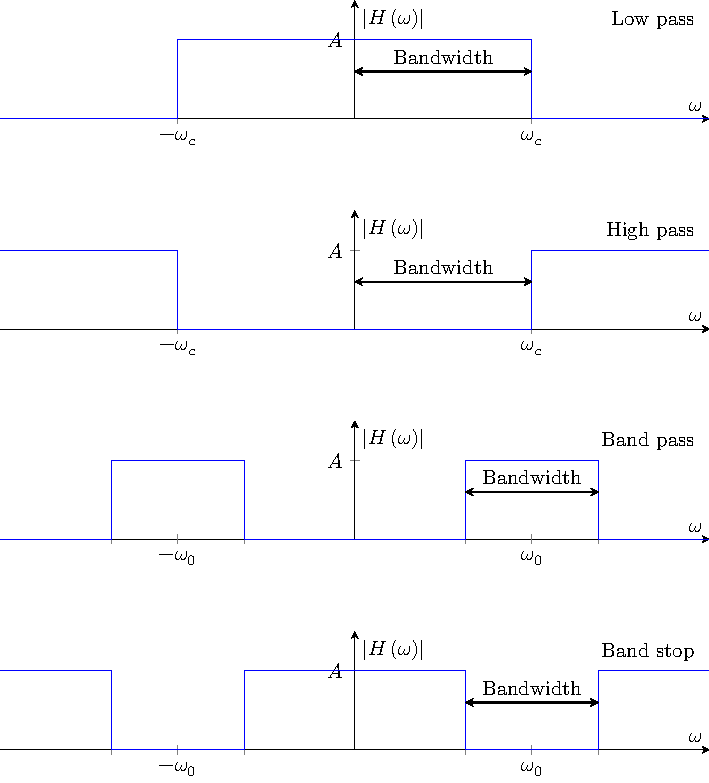
\includegraphics[height = 10cm]{figures/filters.pdf}
    \caption{Magnitude spectra of various ideal filters.} % \label{}
\end{figure}
\subsection{Ideal Filters}
An ideal low/high pass filter only allows frequencies below/above a \textbf{cut-off frequency} \(f_c\) to pass.
This is achieved by setting the transfer function to zero for frequencies above/below the cut-off frequency.

An ideal band pass/stop filter only allows frequencies within a range of frequencies to pass/stop.
These frequencies are centred at a \textbf{center frequency} \(f_0\) and have a \textbf{bandwidth} which is the width of the pass/stop regions.

Ideal filters attenuate completely in their stop bands, and pass signals completely in their pass bands,
and have no effect on the phase of the signal.
\subsection{Practical Filters}
In practice, ideal filters are not realisable because they have infinite attenuation in the stop band.
An ideal filter usually has a \textbf{transition region} between the pass and stop bands.
As this roll-off is not instantaneous, the cut-off frequency and bandwidth of the filter are determined using the \qty{3}{dB} point where
the attenuation is \(\frac{1}{\sqrt{2}}\):
\begin{equation*}
    \abs*{H\left( \omega \right)} = \frac{1}{\sqrt{2}}
\end{equation*}
where \(\omega = 2\pi f\) is the angular frequency.
Consider the second order parallel RLC circuit with transfer function:
\begin{equation*}
    H\left( \omega \right) = \frac{1}{\frac{1}{R} + j \left( \omega C - \frac{1}{\omega L} \right)}
\end{equation*}
The \textbf{resonance frequency} is the frequency at which the transfer function is at its maximum:
\begin{equation*}
    \omega_0 = \frac{1}{\sqrt{LC}}
\end{equation*}
and the bandwidth is given by:
\begin{equation*}
    B = \frac{1}{RC}
\end{equation*}
The \textbf{Q factor} is the ratio of the resonance frequency to the bandwidth:
\begin{equation*}
    Q = \frac{\omega_0}{B}
\end{equation*}
which describes the sharpness of the peak in the magnitude response.
For the parallel RLC circuit, the Q factor is given by:
\begin{equation*}
    Q = R \sqrt{\frac{C}{L}}
\end{equation*}
so that increasing \(R\) increases the Q factor.
\section{Laplace Transform}
When signals are neither periodic nor sinusoidal, the Fourier transform cannot be used.
Any sudden change in a signal is regarded as a transient which disturbs the steady-state operation of a system.
The Laplace transform is a generalisation of the Fourier transform used to determine the response of a system under both
transient and steady-state conditions.
\subsection{Definition}
The two-sided Laplace transform of a function \(f\left( t \right)\) is given by:
\begin{equation*}
    F\left( s \right) = \mathscr{L}\left\{ f\left( t \right) \right\} = \int_{-\infty}^\infty f\left( t \right) e^{-st} \odif{t}
\end{equation*}
where \(s = \sigma + j \omega\) is a complex variable for \(\sigma, \omega \in \R\).
For causal systems, the lower limit of integration is zero.
The inverse Laplace transform is given by:
\begin{equation*}
    f\left( t \right) = \mathscr{L}^{-1}\left\{ F\left( s \right) \right\} = \frac{1}{2\pi j} \int_{\sigma - j\infty}^{\sigma + j\infty} F\left( s \right) e^{st} \odif{s}
\end{equation*}
where \(\sigma\) must be inside the \textbf{text}, which is the
set of complex numbers for which the inverse Laplace transform is defined.

For a causal system, \(\sigma\) is to the right of the pole with the largest real part,
whereas for a non-causal system it is in the vertical strip between two poles.

Note that we typically use tables and partial fraction decomposition to find the inverse Laplace transform.
\subsection{Conditions for Existence}
The Laplace transform converges when
\begin{equation*}
    \int_{-\infty}^\infty \abs*{f\left( t \right) e^{-\sigma t}} \odif{t} < \infty
\end{equation*}
for finite \(\sigma\). Or equivalently when,
\begin{equation*}
    \lim_{t \to \infty} f\left( t \right) e^{-s t} = 0.
\end{equation*}
\subsection{Laplace Transform Properties}
Like the Fourier transform, many properties of the Laplace transform can be derived from the definition.
Notably, the Laplace transform is linear and also satisfies the convolution theorem.
\subsection{Zeros and Poles}
The zeros and poles of a function \(f\left( t \right)\) are the roots of the numerator and denominator of its Laplace transform.
\subsection{Circuit Analysis}
Two common circuits are the RC and RL circuits.
\begin{figure}[H]
    \centering
    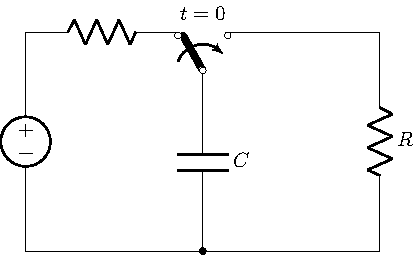
\includegraphics[height = 4cm]{figures/rc_natural.pdf}
    \caption{RC circuit.} % \label{}
    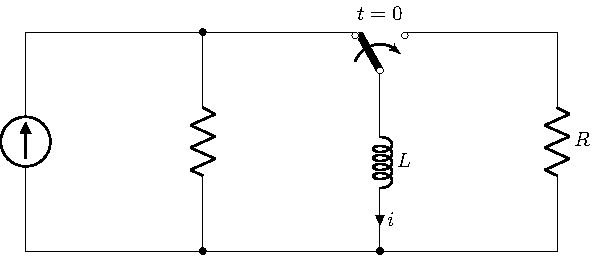
\includegraphics[height = 4cm]{figures/rl_natural.pdf}
    \caption{RL circuit.} % \label{}
\end{figure}
For an RC circuit:
\begin{equation*}
    v\left( t \right) = v\left( 0 \right) e^{-t/\tau}
\end{equation*}
with \(\tau = RC\).
\begin{figure}[H]
    \centering
    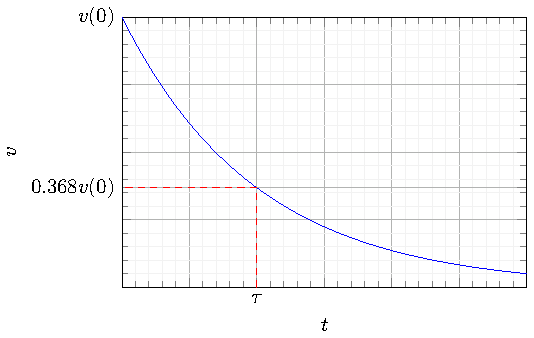
\includegraphics[height = 4cm]{figures/rc_natural_plot.pdf}
    \caption{Natural response of RC circuit.} % \label{}
\end{figure}
For an RL circuit:
\begin{equation*}
    i\left( t \right) = i\left( 0 \right) e^{-t/\tau}
\end{equation*}
with \(\tau = \frac{1}{R}L\).
\begin{figure}[H]
    \centering
    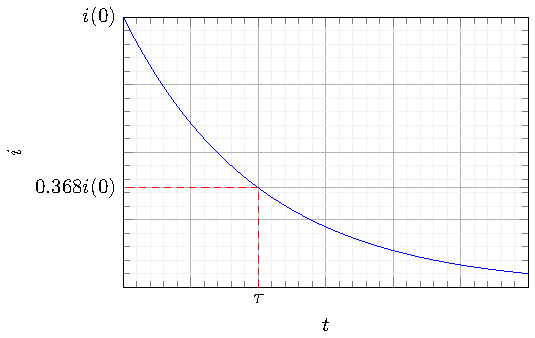
\includegraphics[height = 4cm]{figures/rl_natural_plot.pdf}
    \caption{Natural response of RL circuit.} % \label{}
\end{figure}
\(\tau\) is the time constant that describes the time taken for the response to decay to \(1/e\) of its initial value.

For the step responses, consider the following circuits:
\begin{figure}[H]
    \centering
    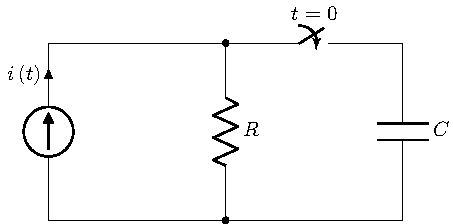
\includegraphics[height = 4cm]{figures/rc_step.pdf}
    \caption{RC circuit.} % \label{}
    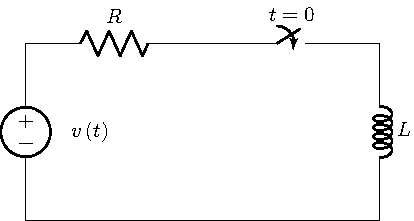
\includegraphics[height = 4cm]{figures/rl_step.pdf}
    \caption{RL circuit.} % \label{}
\end{figure}
For an RC circuit:
\begin{equation*}
    v\left( t \right) = v\left( \infty \right) + \left[ v\left( 0^{+} \right) - v\left( \infty \right) \right] e^{-t/\tau}
\end{equation*}
\begin{figure}[H]
    \centering
    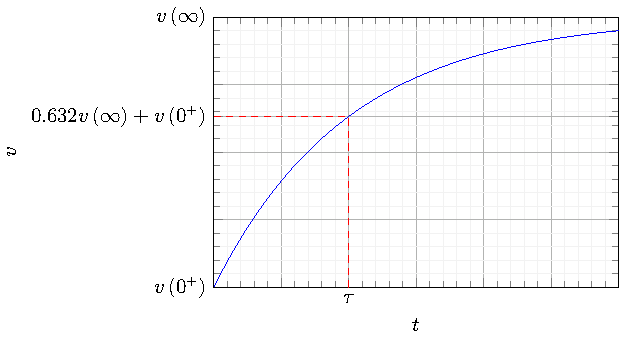
\includegraphics[height = 4cm]{figures/rc_step_plot.pdf}
    \caption{Step response of an RC circuit.} % \label{}
\end{figure}
For an RL circuit:
\begin{equation*}
    i\left( t \right) = i\left( \infty \right) + \left[ i\left( 0^{+} \right) - i\left( \infty \right) \right] e^{-t/\tau}
\end{equation*}
\begin{figure}[H]
    \centering
    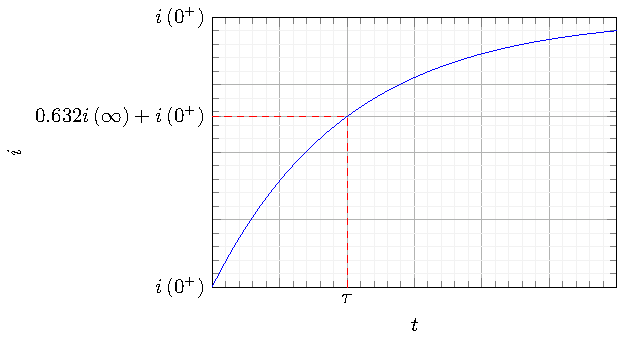
\includegraphics[height = 4cm]{figures/rl_step_plot.pdf}
    \caption{Step response of an RL circuit.} % \label{}
\end{figure}
where \(v\left( \infty \right)\) and \(i\left( \infty \right)\) are the steady-state values of the voltage and current respectively.
To determine the initial and steady-state values of the voltage and current, we can use the Laplace transform.
\subsection{Initial and Final Value Theorems}
If the poles of \(F\left( s \right)\) are in the left hand side of the \(s\)-plane, the system is \textbf{stable}.
Given a stable system,
\begin{align*}
    f\left( 0^{+} \right)  & = \lim_{s \to \infty} s F\left( s \right) \\
    f\left( \infty \right) & = \lim_{s \to 0} s F\left( s \right)
\end{align*}
\subsection{Impedance}
The impedance of an element is the ratio of the voltage to the current.
Consider the capacitor and inductor definitions:
\begin{align*}
    i\left( t \right) & = C \odv{v}{t} \\
    v\left( t \right) & = L \odv{i}{t}
\end{align*}
taking the Laplace transform gives:
\begin{align*}
    I\left( s \right) & = sC V\left( s \right) \\
    V\left( s \right) & = sL I\left( s \right)
\end{align*}
where we assume that the initial conditions are zero. This gives us an \(s\)-domain definition of impedance for reactive elements:
\begin{align*}
    Z_C & = \frac{1}{sC} \\
    Z_L & = sL
\end{align*}
These definitions allow us to analyse circuits by first applying
the Laplace transform to all elements and solving the circuit via Kirchhoff's laws either through mesh or nodal analysis.
\subsection{Common Filters}
Using the above definitions, we can derive the transfer functions of common RC/RL filters.
Here \(\omega_c = 1/\tau\) is the cut-off (angular) frequency.
\subsubsection{RC Low Pass Filter}
\begin{figure}[H]
    \centering
    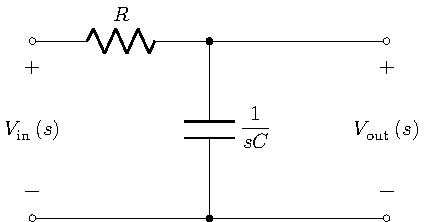
\includegraphics[height = 4cm]{figures/rc_low_pass_filter.pdf}
    \caption{RC low pass filter.} % \label{}
\end{figure}
The transfer function of the RC low pass filter is:
\begin{align*}
    H\left( s \right) & = \frac{\frac{1}{sC}}{R + \frac{1}{sC}} & \left( \times \frac{s/R}{s/R} \right) \\
                      & = \frac{\frac{1}{RC}}{s + \frac{1}{RC}}                                         \\
                      & = \frac{\omega_c}{s + \omega_c}
\end{align*}
with \(\omega_c = \frac{1}{RC}\).
\subsubsection{RC High Pass Filter}
\begin{figure}[H]
    \centering
    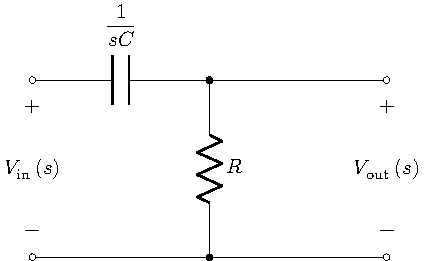
\includegraphics[height = 4cm]{figures/rc_high_pass_filter.pdf}
    \caption{RC high pass filter.} % \label{}
\end{figure}
The transfer function of the RC high pass filter is:
\begin{align*}
    H\left( s \right) & = \frac{R}{\frac{1}{sC} + R} & \left( \times \frac{s/R}{s/R} \right) \\
                      & = \frac{s}{\frac{1}{RC} + s}                                         \\
                      & = \frac{s}{\omega_c + s}
\end{align*}
with \(\omega_c = \frac{1}{RC}\).
\subsubsection{RL Low Pass Filter}
\begin{figure}[H]
    \centering
    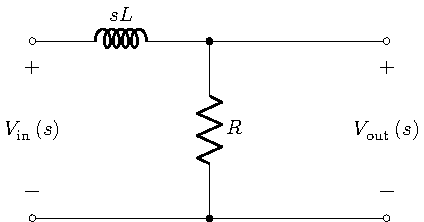
\includegraphics[height = 4cm]{figures/rl_low_pass_filter.pdf}
    \caption{RL low pass filter.} % \label{}
\end{figure}
The transfer function of the RL low pass filter is:
\begin{align*}
    H\left( s \right) & = \frac{R}{sL + R}            & \left( \times \frac{1/R}{1/R} \right) \\
                      & = \frac{1}{s\frac{1}{R}L + 1}                                         \\
                      & = \frac{1}{s\omega_c + 1}
\end{align*}
with \(\omega_c = \frac{1}{\frac{1}{R}L}\).
\subsubsection{RL High Pass Filter}
\begin{figure}[H]
    \centering
    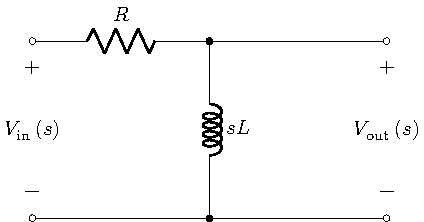
\includegraphics[height = 4cm]{figures/rl_high_pass_filter.pdf}
    \caption{RL high pass filter.} % \label{}
\end{figure}
The transfer function of the RL high pass filter is:
\begin{align*}
    H\left( s \right) & = \frac{sL}{R + sL}                       & \left( \times \frac{1/R}{1/R} \right) \\
                      & = \frac{s\frac{1}{R}L}{1 + s\frac{1}{R}L}                                         \\
                      & = \frac{s}{1 + s\omega_c}
\end{align*}
with \(\omega_c = \frac{1}{\frac{1}{R}L}\).
\section{Quantisation}
Digital signals are discrete in both time and amplitude. A
\textbf{quantiser} transforms each sampled value to take one of \(L\) distinct levels.
The \(L\) levels are allocated over the entire dynamic range of the analog signal
\begin{equation*}
    x_\mathrm{min} \leq x\left( t \right) \leq x_\mathrm{max}
\end{equation*}
This procedure is non-invertible.
\subsection{Uniform Quantisers}
A uniform quantiser divides the \textbf{dynamic range} (\(x_\mathrm{max} - x_\mathrm{min}\)) into \(L\) equal intervals,
known as \textbf{quantisation levels}.

The step size \(\Delta\) between quantisation levels is calculated by
\begin{equation*}
    \Delta = \frac{x_\mathrm{max} - x_\mathrm{min}}{L}
\end{equation*}
Many applications have \(x_\mathrm{max} = -x_\mathrm{min}\), so the step size is
\begin{equation*}
    \Delta = \frac{2 x_\mathrm{max}}{L}
\end{equation*}
The number of levels \(L\) is usually a power of two,
\begin{equation*}
    L = 2^n
\end{equation*}
where \(n\) is the number of bits to encode \(L\) levels.

\end{document}
